\documentclass[../../main.tex]{subfiles}

\graphicspath{{../../image/}{../../figure/}}

\begin{document}

\section{风格迁移}\label{section:ch10-风格迁移}

深度卷积网络中的早期层学习检测边缘和纹理等简单特征，而后续层则学习检测更复杂的对象等实体（参见\cref{section:ch10-可视化训练好的CNN}）。我们可以利用这一性质，使用一种称为神经风格迁移（neural style transfer）的过程来以另一种图像的风格重新渲染图像（Gatys, Ecker, and Bethge, 2015），如\cref{figure:ch10-风格迁移}所示。

\begin{figure}[htbp]
  \centering
  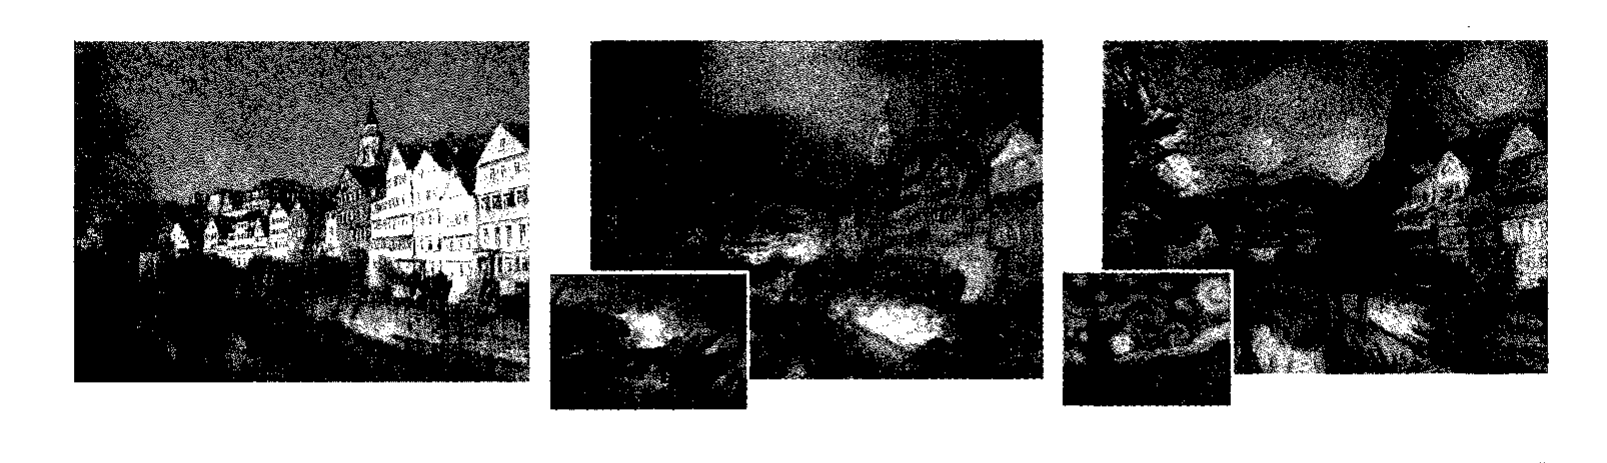
\includegraphics[width=0.95\textwidth]{ch10-fig10-32-风格迁移.png}
  \caption{一个神经风格迁移的示例，展示了一张运河场景的照片（左）以 J.\,M.\,W.\ Turner 的《运输船遇难》（中）风格和 Vincent van Gogh 的《星月夜》（右）风格渲染后的效果，用于提供样式的图像都显示在小图中［经 Gatys, Ecker and Bethge (2015) 授权使用］。}
  \label{figure:ch10-风格迁移}
\end{figure}

我们的目标是生成合成图像 $G$，其“内容”由图像 $C$ 定义，其“风格”来自另一幅图像 $S$。这可以通过定义由以下两项的和组成的误差函数 $E(G)$ 来实现，其中一项促使 $G$ 具有与 $C$ 相似的内容，另一项则促使 $G$ 具有与 $S$ 相似的风格：
\begin{align}
  E(G)=E_{\mathrm{content}}(G,C)+E_{\mathrm{style}}(G,S).
  \label{align:ch10-风格迁移总误差}
\end{align}
图像内容和风格的概念由这两项的函数形式隐含定义。然后，我们可以通过从随机初始化的图像开始，并使用梯度下降最小化 $E(G)$ 来得到 $G$。

\begin{definition}[神经风格迁移]\label{definition:ch10-风格迁移}
设 $C$ 为内容图像、$S$ 为风格图像，$E_{\mathrm{content}}$ 与 $E_{\mathrm{style}}$ 为给定的内容误差与风格误差，$E$ 由\eqref{align:ch10-风格迁移总误差}定义。称从随机初始化的图像出发、用梯度下降最小化 $E(G)$ 而得到的图像 $G$ 为以 $C$ 为内容、$S$ 为风格的\textbf{神经风格迁移}结果，称这一过程为神经风格迁移（neural style transfer）。
\end{definition}

% SUPPLEMENT: parent=definition:ch10-风格迁移; kind=motivation; location=紧随其后的 remark（重构新增）
\begin{remark}（重构新增）
这个定义的关键在于它并不定义“内容”与“风格”这两个词本身，而是通过两个误差项的函数形式隐含地定义它们：凡是被 $E_{\mathrm{content}}$ 约束的，就是内容；凡是被 $E_{\mathrm{style}}$ 约束的，就是风格。因此换一种误差项的函数形式，就等于换了一种对“风格”的理解，这不是实现细节而是模型定义的一部分。定义要求从随机图像出发并使用梯度下降，说明 $G$ 是优化变量而不是网络参数：网络本身是固定的特征提取器（通常是预训练的 VGG），被优化的是像素。这个选择带来一个实践上的后果：每生成一幅图都要重新求解一次优化问题，速度远慢于训练一个前馈生成网络。
\end{remark}

为了定义 $E_{\mathrm{content}}(G,C)$，我们可以选择网络中特定的卷积层，并将图像 $G$ 用作输入，计算该层中单元的激活，对图像 $C$ 也执行相同的操作。然后我们可以促使相应的预激活值变得相似，方法是使用如下形式的平方和误差函数：
\begin{align}
  E_{\mathrm{content}}(G,C)=\sum_{i,j,k}\left(a_{ijk}(G)-a_{ijk}(C)\right)^2,
  \label{align:ch10-内容误差}
\end{align}
其中 $a_{ijk}(G)$ 表示当输入图像为 $G$ 时，该层中通道 $k$ 位置 $(i,j)$ 处单元的预激活值；类似地，$a_{ijk}(C)$ 表示当输入图像为 $C$ 时，该层中通道 $k$ 位置 $(i,j)$ 处单元的预激活值。选择哪层用于定义预激活会影响最终结果，早期层旨在匹配边缘等低级特征，后续层则旨在匹配更复杂的结构甚至整个对象。

在定义 $E_{\mathrm{style}}(G,S)$ 时，直觉上图像风格是由卷积层中不同通道的特征共现来确定的。例如，如果风格图像 $S$ 中的垂直边缘通常与橙色斑块相关联，那么我们希望生成的图像 $G$ 也是如此。然而，尽管 $E_{\mathrm{content}}(G,C)$ 尝试匹配 $G$ 的特征与 $C$ 中相同位置的相应特征，但对于风格误差 $E_{\mathrm{style}}(G,S)$，我们希望 $G$ 具有与 $S$ 相匹配的特征，因此我们选择对特征图中的位置取平均。与之前一样，考虑一个特定的卷积层。我们可以通过构建互相关矩阵来衡量输入图像 $G$ 的通道 $k$ 中的特征与通道 $k'$ 中相应特征的共现程度：
\begin{align}
  F_{kk'}(G)=\sum_{i=1}^{I}\sum_{j=1}^{J}a_{ijk}(G)\,a_{ijk'}(G),
  \label{align:ch10-Gram矩阵}
\end{align}
其中，$I$ 和 $J$ 是这个特定卷积层中特征图的维度，乘积 $a_{ijk}a_{ijk'}$ 在两个特征均激活时值较大。如果该层有 $K$ 个通道，则 $F_{kk'}$ 形成一个 $K\times K$ 的矩阵，称为风格矩阵（style matrix）。我们可以通过使用下式比较它们的风格矩阵来衡量图像 $G$ 和 $S$ 具有相同风格的程度：
\begin{align}
  E_{\mathrm{style}}(G,S)=\frac{1}{(2IJK)^2}\sum_{k=1}^{K}\sum_{k'=1}^{K}\left(F_{kk'}(G)-F_{kk'}(S)\right)^2.
  \label{align:ch10-风格误差}
\end{align}
虽然也可以使用单层，但通过使用以下形式多层的贡献可以获得更令人满意的结果：
\begin{align}
  E_{\mathrm{style}}(G,S)=\sum_{l}\lambda_l E_{\mathrm{style}}^{(l)}(G,S),
  \label{align:ch10-多层风格误差}
\end{align}
其中，$l$ 表示卷积层。系数 $\lambda_l$ 不仅确定了不同层之间的相对权重，也确定了相对于内容误差项的权重。这些权重系数是由主观判断经验性地调整的。

\begin{definition}[风格矩阵（Gram 矩阵）]\label{definition:ch10-Gram矩阵}
设某卷积层有 $K$ 个通道、每个通道的空间尺寸为 $I\times J$，$a_{ijk}$ 为通道 $k$ 在位置 $(i,j)$ 的预激活。称由\eqref{align:ch10-Gram矩阵}定义的 $K\times K$ 矩阵 $F(G)=(F_{kk'}(G))$ 为输入图像 $G$ 在该层的\textbf{风格矩阵}（style matrix），亦称 \textbf{Gram 矩阵}。
\end{definition}

% SUPPLEMENT: parent=definition:ch10-Gram矩阵; kind=motivation; location=紧随其后的 remark（重构新增）
\begin{remark}（重构新增）
风格矩阵把“某层特征图”压缩成一个 $K\times K$ 的通道间相关矩阵，其代价是彻底丢弃空间信息：$F_{kk'}$ 对全部位置求和，因此两幅图只要通道间的共现统计相同，风格矩阵就相同，哪怕图案排布完全不同。这正是“风格”与“内容”的分界：内容误差\eqref{align:ch10-内容误差}逐位置比较，风格误差\eqref{align:ch10-风格误差}只比较统计量。定义中“对位置求和”而不是取平均，使 $F$ 的数值随特征图尺寸增大而增大，故\eqref{align:ch10-风格误差}前的归一化因子 $(2IJK)^2$ 不是装饰：没有它，不同层的误差量级会随分辨率剧烈变化，$\lambda_l$ 就无法跨层比较。
\end{remark}

\begin{proposition}[Gram 矩阵的基本性质]\label{proposition:ch10-Gram矩阵性质}
设 $A\in\mathbb{R}^{IJ\times K}$ 的列是各通道展平后的向量，则 $F=A^{\mathsf{T}}A$。于是
\begin{enumerate}
  \item $F$ 对称：$F^{\mathsf{T}}=F$；
  \item $F$ 半正定：对任意 $\mathbf{v}\in\mathbb{R}^{K}$ 有 $\mathbf{v}^{\mathsf{T}}F\mathbf{v}\geqslant0$，且等号成立当且仅当 $A\mathbf{v}=\mathbf{0}$；
  \item $\operatorname{rank}(F)=\operatorname{rank}(A)\leqslant\min\{IJ,K\}$。
\end{enumerate}
\end{proposition}
\begin{proof}
把 $F_{kk'}=\sum_{i,j}a_{ijk}a_{ijk'}$ 写成向量内积，正是 $A$ 的第 $k$ 列与第 $k'$ 列的内积，故 $F=A^{\mathsf{T}}A$。(1) $F^{\mathsf{T}}=(A^{\mathsf{T}}A)^{\mathsf{T}}=A^{\mathsf{T}}A=F$。(2) $\mathbf{v}^{\mathsf{T}}F\mathbf{v}=\mathbf{v}^{\mathsf{T}}A^{\mathsf{T}}A\mathbf{v}=\|A\mathbf{v}\|^2\geqslant0$，而 $\|A\mathbf{v}\|^2=0$ 当且仅当 $A\mathbf{v}=\mathbf{0}$。(3) 由 $\operatorname{rank}(A^{\mathsf{T}}A)=\operatorname{rank}(A)$ 及 $\operatorname{rank}(A)\leqslant\min\{IJ,K\}$ 即得。证毕。
\end{proof}

% SUPPLEMENT: parent=proposition:ch10-Gram矩阵性质; kind=motivation; location=紧随其后的 remark（重构新增）
\begin{remark}（重构新增）
这三个性质各有用途。对称性使 $F$ 只有 $K(K+1)/2$ 个独立元素，风格误差实际比较的自由度比 $K^2$ 少。半正定性保证了 $F$ 可以看作某个特征分布的协方差矩阵，因此“风格距离”在统计意义上是有依据的；但要注意 $F$ 通常奇异（当 $IJ>K$ 时秩至多为 $K$，更常见的是通道间高度相关），所以不能直接求逆，任何用到 $F^{-1}$ 的写法都需要正则化。秩的上界说明风格矩阵能表达的相关性受通道数限制：通道太少时，丰富的纹理统计无法被完整编码。第 (2) 条的等号条件在数值上意味着：若某线性组合 $A\mathbf{v}$ 在全部位置上为零，则 $F$ 在该方向上退化，这通常出现在某通道恒为零（例如 ReLU 之后整片失活）的情形。
\end{remark}

\end{document}
